%\input{./sbchead}

%%%% Proceedings format for most of ACM conferences (with the exceptions listed below) and all ICPS volumes.
%\documentclass[sigconf]{acmart}
\documentclass{sig-alternate}
%%%% As of March 2017, [siggraph] is no longer used. Please use sigconf (above) for SIGGRAPH conferences.

%%%% Proceedings format for SIGPLAN conferences 
% \documentclass[sigplan, anonymous, review]{acmart}

%%%% Proceedings format for SIGCHI conferences
% \documentclass[sigchi, review]{acmart}

%%%% To use the SIGCHI extended abstract template, please visit
% https://www.overleaf.com/read/zzzfqvkmrfzn


\usepackage{booktabs} % For formal tables

%\usepackage{cite}
\usepackage{amsmath,amssymb,amsfonts}
\usepackage{algorithmic}
\usepackage{textcomp}
\usepackage[utf8]{inputenc}
\usepackage[T1]{fontenc}
\usepackage{float}

\usepackage[brazil]{babel}   
%\usepackage[latin1]{inputenc}  
% UTF-8 encoding is recommended by ShareLaTex


%\usepackage[x11names,dvipsnames,table]{xcolor} 
\usepackage{array}
\newcolumntype{L}[1]{>{\raggedright\let\newline\\\arraybackslash\hspace{0pt}}m{#1}}
\newcolumntype{C}[1]{>{\centering\let\newline\\\arraybackslash\hspace{0pt}}m{#1}}
\newcolumntype{R}[1]{>{\raggedleft\let\newline\\\arraybackslash\hspace{0pt}}m{#1}}
\usepackage{multirow}
\usepackage{hyperref}
\usepackage{url}

\usepackage{amsmath}


\newcolumntype{P}[1]{>{\centering\arraybackslash}p{#1}}
\usepackage{booktabs}
\usepackage{graphicx}

\sloppy
%\usepackage{natbib}
%\usepackage{graphicx}




% These commands are optional
%\acmBooktitle{Transactions of the ACM Woodstock conference}
%\editor{Jennifer B. Sartor}
%\editor{Theo D'Hondt}
%\editor{Wolfgang De Meuter}


\begin{document}
\title{Mapeando Abordagens de Design de Front-End para Model-Driven Web Engineering}
\title{Mapping Front End Design Approaches for Model-Driven Web Engineering}
\subtitle{Alternative Title: Mapping Model-Driven Web Engineering Front-End Design Approaches}
%\titlenote{Produces the permission block, and copyright information}
%\subtitle{...}
%\subtitlenote{The full version of the author's guide is available as
%  \texttt{acmart.pdf} document}

%\author{Jean T. Piagetti, Maurício El Uri, Fábio Paulo Basso, Elder de Macedo Rodrigues, Maicom Bernardino da Silveira}
%\affiliation{%
%  \institution{Universidade Federal do Pampa (UNIPAMPA), Engenharia de Software}
%  \streetaddress{ Av. Tiarajú, 810 - Bairro: Ibirapuitã}
%  \city{Alegrete}
%  \state{Rio Grande do Sul, Brazil}
%  \postcode{97546-550}
%}
%\email{mauricioeluri,jeanpiagetti@gmail.com}
%\email{fabiobasso@unipampa.edu.br}





%\author{Lars Th{\o}rv{\"a}ld}
%\authornote{This author is the
%  one who did all the really hard work.}
%\affiliation{%
%  \institution{The Th{\o}rv{\"a}ld Group}
%  \streetaddress{1 Th{\o}rv{\"a}ld Circle}
%  \city{Hekla}
%  \country{Iceland}}
%\email{larst@affiliation.org}

%\author{Valerie B\'eranger}
%\affiliation{%
%  \institution{Inria Paris-Rocquencourt}
%  \city{Rocquencourt}
%  \country{France}
%}
%\author{Aparna Patel}
%\affiliation{%
% \institution{Rajiv Gandhi University}
% \streetaddress{Rono-Hills}
% \city{Doimukh}
% \state{Arunachal Pradesh}
% \country{India}}
%\author{Huifen Chan}
%\affiliation{%
%  \institution{Tsinghua University}
%  \streetaddress{30 Shuangqing Rd}
%  \city{Haidian Qu}
%  \state{Beijing Shi}
%  \country{China}
%}

%\author{Charles Palmer}
%\affiliation{%
%  \institution{Palmer Research Laboratories}
%  \streetaddress{8600 Datapoint Drive}
%  \city{San Antonio}
%  \state{Texas}
%  \postcode{78229}}
%\email{cpalmer@prl.com}

%\author{John Smith}
%\affiliation{\institution{The Th{\o}rv{\"a}ld Group}}
%\email{jsmith@affiliation.org}

%\author{Julius P.~Kumquat}
%\affiliation{\institution{The Kumquat Consortium}}
%\email{jpkumquat@consortium.net}

% The default list of authors is too long for headers.
%\renewcommand{\shortauthors}{B. Trovato et al.}


\maketitle

%%%%%%
% Use esse ambiente apenas se o artigo for em Português.
%%%%%%

%\begin{resumo}
%Este artigo caracteriza 38 estudos, publicados entre 2005 e 2018, endereçando o desenvolvimento de web front-ends por meio de ferramentas para Model-Driven Web Engineering (MDWE). Ele aborda Linguagens Específicas de Domínio (DSLs), com o uso de técnicas de design, propostas para auxiliar em muitas fases de desenvolvimento de software. Também aborda quais destas ferramentas são caracterizadas para prototipagem rápida de aplicações, com prototipação evolutiva e geração de código fonte, que tem como objetivo acelerar o processo de de análise por meio de design automático. Nossa conclusão é que apenas seis destas propostas têm sido relatadas com aplicação na indústria, assim uma limitação encontrada na literatura da área que atrapalha a compreensão dos critérios de aceitação destas ferramentas em contextos de fábricas de software. 
%\end{resumo}

%%%%%%
% Use esse comando apenas se o artigo for em Português
%%%%%%
%\palavraschave{Mockup, Web Front-End, DSL, MDE, Mapeamento Sistemático}

\begin{abstract}
This paper characterizes 38 studies, published between 2005 and 2018, scoping the development of web front-ends through toolboxes for Model-Driven Web Engineering (MDWE). It addresses Domain Specific Languages (DSLs), embedded with some design techniques, devoted to help in the various phases of software development. Moreover, it also contextualizes model-based tools for rapid prototyping, with evolutive prototyping and source code generation, and highligths those that speed-up the analysis process through automated design. Our conclusion is that only six of these studies have been reported to be executed in industry, thus a limitation found in the literature of the area that hinders the understanding of the acceptance criteria of these tools in contexts of software factories.%thus a limitation for understanding acceptance criterias calling for new empirical studies in Software Engineering.
\end{abstract}

% A category with the (minimum) three required fields
\category{H.4}{Information Systems Applications}{Miscellaneous}
%A category including the fourth, optional field follows...
\category{D.2.2}{Software Engineering}{Design Tools and Techniques}[Computer-aided software engineering (CASE), User interfaces]

%\terms{Theory}

\keywords{Mockup, Web Front-End, Domain Specific Language, Model-Driven Engineering, Systematic Mapping Study}





\section{Introdução}
Temos visto cada vez mais esforços para tornar o conteúdo presente na internet acessível aos usuários finais. Porém, mesmo com todos estes esforços, poucos programadores e equipes de desenvolvimento realmente se preocupam em tornar seus websites acessíveis em múltiplas plataformas~\cite{Brambilla14,Rivero2017}. Por exemplo, além do conhecimento técnico necessário para desenvolvimento de sistemas de informação~\cite{Basso16JSS}, desafios para incorporar em aplicativos as novidades do mercado incluem, principalmente, a dificuldade das equipes de desenvolvimento de cumprir com o cronograma em iterações de um processo de desenvolvimento cada vez mais curtas~\cite{OLIVEIRA201886}. Por conta disso, importantes características de um sistema web como acessibilidade, facilidade de uso e navegabilidade acabam ficando de lado em prol de cumprir com o escasso tempo de mercado. 

Neste sentido, ferramentas para Prototipação Rápida de Aplicações (RAP)~\cite {Elkoutbi06, Planas09} podem contribuir para superar este desafio. Algumas destas ferramentas permitem, por meio de modelos, a geração de sistemas conforme múltiplas plataformas~\cite{Vara12}. Para tanto, Model-Driven Engineering (MDE)~\cite{Kent02} é um paradigma para o desenvolvimento de software baseado em transformações de modelos, e vem sendo implementado com algumas técnicas de design que contribuem para a RAP. 

Em processos típicos baseados em MDE, as transformações de modelo devem receber um modelo altamente detalhado para gerar partes funcionais de aplicativos~\cite {Schmidt06}. Para gerar o código-fonte completo~\cite{Kelly08}, várias partes de um design de aplicativo são detalhadas em DSLs (Domain Specific Languages)~\cite{Voelter09} e/ ou decoradas com anotações adicionadas aos elementos de modelo representados com a UML (Unified Modeling Language)~\cite{Elkoutbi06}, uma linguagem de modelagem de propósito geral usada em projetos arquiteturais de alguns sistemas web. Em qualquer caso, isso torna a construção do software dependente de tarefas de design.

Neste contexto, nosso objetivo é descrever 13 anos de pesquisa no design de front-end web focando em Model-Driven Web-Engineering (MDWE). MDWE inclui desde abordagens para arquitetura de redes de computadores ao desenvolvimento de aplicativos web~\cite{Brambilla14}. Assim, focamos este estudo nas DSLs propostas para design de front-ends web e nas abordagens que automatizam o design por meio de transformações de modelos~\cite{Batory13MODELS}. 

A seguir apresenta-se o resultado do nosso mapeamento. Inicialmente, a Seção~\ref{sec:embteorico} apresenta um embasamento teórico sobre abordagens para Model-Driven Web Engineering. A Seção~\ref{sec:method} introduz o método de pesquisa adotado para o planejamento e execução deste mapeamento sistemático de literatura. A Seção~\ref{sec:stateoftheart} relata achados deste mapeamento, complementado pela Seção~\ref{sec:threats} com ameaças à validade do estudo. Finalmente, a Seção~\ref{sec:conclusions} apresenta nossas conclusões e trabalhos futuros.

\section{Embasamento Teórico}
\label{sec:embteorico}

No desenvolvimento de sistemas de informações da web, os front-ends da web como o layout são compostos pelos componentes para GUI (Graphical User Interface)~\cite{MIJAILOVIC2014757} e por diagramas comportamentais~\cite{Nunes06}. Para permitir a geração de código-fonte completo com uma abordagem MDWE, esses modelos são decorados com a semântica para ações do usuário, fluxos de tela e lógica de negócios. Assim, usando-se uma DSL apropriada, é possível abstrair detalhes de implementação, focando na especificação de semântica em modelos que formalizam o conhecimento sobre requisitos de software. % ~\cite{France01}.

\begin{figure*}[ht!]
    \centering
    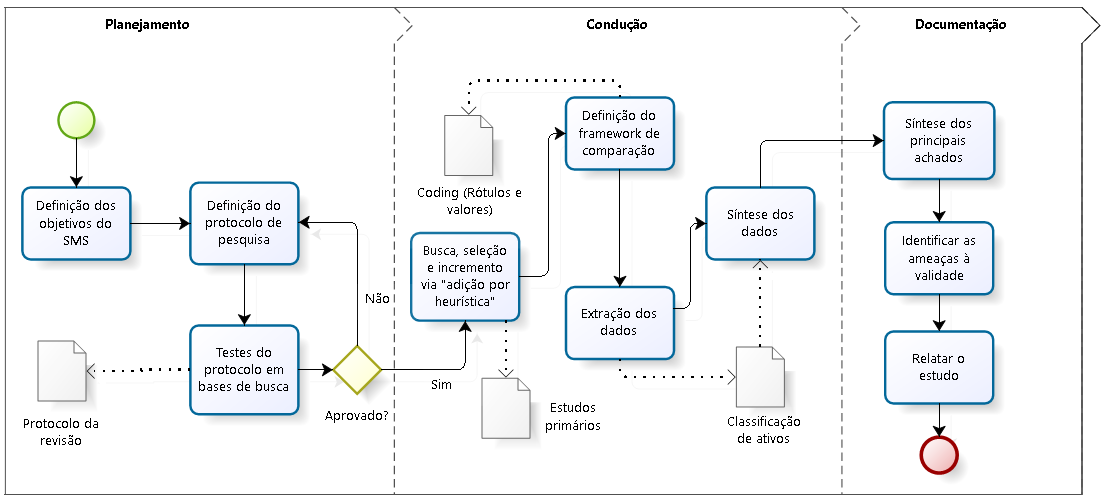
\includegraphics[width=540pt]{./mdweresearchmethod.png}
    \caption{Metodologia de pesquisa.}
    \label{fig:method}
\end{figure*}
%É apresentado um estudo de caso ~\cite{toala2018evaluating} de o porquê da não, ou baixa, adoção do MDWE para desenvolvimento de sistemas web.A análise é feita levando em consideração aspectos da personalidade do desenvolvedor(extroversão, neuroticismo(ansiedade) e ceticismo) que podem contribuir para o baixo uso MDWE.Como resultados obtidos, mostra que os indivíduos neuroticistas influenciam a usabilidade do MDWE 

O MDWE permite o desenvolvimento de sistemas de informação para múltiplas plataformas por meio de transformações de modelos~\cite{Vara12}. Outro emprego comum, por exemplo, é no desenvolvimento de serviços que integram múltiplos sistemas (mashups), usando uma arquitetura orientada a serviço (SOA) e também micro-serviços~\cite{DEVRIEZE2011637}. Por fim, outro bom exemplo está na automação de processos de negócios, realizada por meio de modelos representados com BPMN~\cite{Pillat15}. %, como o acoplamento dessas aplicações é baixo, significa que as funcionalidades podem ser trabalhadas separadamente, essa abordagem tende a melhorar a agilidade e a produtividade.   


Uma ampla variedade de abordagens para MDWE foram propostas como produtos derivados de pesquisa desde 2000~\cite{Ceri00}. Atualmente, a falta de um mapeamento das propostas existentes gera uma incerteza sobre o que cada ferramenta oferece para a indústria de software, bem como quais são as lacunas de pesquisa. Assim, este estudo apresenta um mapeamento de propostas para MDWE que introduzem elementos representacionais para o design de GUIs que levam à geração de protótipos. Este mapeamento é novo, já que estudos existentes focam em plataformas específicas como AJAX~\cite{mesbah2008component}, com análise de propostas e desafios sobre frameworks mais utilizados. Diferentemente, nosso estudo foca em tecnologia existente para gerar código específico de plataforma por meio de modelos independentes delas.

Um Estudo de Mapeamento Sistemático (SMS)~\cite{Kitchenham07} consiste basicamente em uma investigação para examinar e identificar lacunas de pesquisa, dando uma visão geral sobre o estado da arte e elencando os principais trabalhos publicados na área. %Para alcançá-lo, diversos estudos propõem protocolos rigorosos para a definição das sequências de busca e o processo de seleção dos estudos. As strings de pesquisa são organizadas definindo as principais palavras-chave e seus sinônimos. O processo de busca é composto por no mínimo quatro etapas: definição das questões de pesquisa, uma estratégia de busca (busca de strings, busca de bases para encontrar), critérios de inclusão e exclusão de estudos e, finalmente, os possíveis dados esperados em cada questão de pesquisa. 


\section{Método de Pesquisa}
\label{sec:method}

Várias ferramentas foram propostas como uma maneira de ajudar os engenheiros de software a projetar várias camadas de aplicativos a partir de aplicativos da Web por meio de DSLs dedicadas a recursos estruturais para front-end. Tais ferramentas são construídas com base em muitos conceitos introduzidos em engenharia de software, abrangendo recursos como GUIs, serviços, padrões arquiteturais, padrões de interação e implementações específicas para plataformas. Neste contexto, uma limitação na literatura é a falta de estudos mapeando o estado da arte em abordagens MDWE para o projeto de front-end. Em especial, essa limitação atrapalha a tomada de decisão sobre quais são as características de abordagens relatadas como mais adequadas para determinados contextos, como elementos de DSLs desenvolvidos para as necessidades de times ágeis~\cite{Rivero2014}. Logo, tal limitação motiva a criação de uma visão panorâmica da evolução destas abordagens para problemas que foram surgindo no desenvolvimento de software web.Para superar esta limitação, realizou-se um SMS. 

%Colocar o texto o protocolo com as questões de pesquisa.  
Para a relização deste SMS, uma metodologia de pesquisa foi selecionada~\footnote{Metodologia base <https://arxiv.org/pdf/1611.02619.pdf>} e adaptada para as atividades ilustradas na Figura~\ref{fig:method}. Nela, considera-se os aspectos que englobam o conjunto dos elementos do MDWE em quatro artefatos: 1) Protocolo da revisão, com os elementos discutidos logo mais nesta seção; 2) Estudos primários, um pacote contendo os artigos selecionados; 3) Coding (Rótulos e valores), uma planilha contendo os rótulos que foram extraídos para classificar os trabalhos selecionados, e; 4) Classificação de ativos, um modelo que representa os estudos selecionados como ativos descrevendo recursos intensivos em conhecimento. %Este modelo é representado conforme a DSL RAS++ e segue os critérios de qualidade para descrição de ferramentas de MDE discutidos em~\cite{Basso17b}.






%disponível em <\url{https://docs.google.com/spreadsheets/d/1_GqP38moU0qaIfJ6fnsE5fRG8gEGskbWRttn0C5TNKc/edit#gid=0}>. 





Como por exemplo de critérios de inclusão, podemos citar as ferramentas de prototipagem, design automatizado, DSLs voltadas para desenvolvimento web, RAP-Prototipação rápida de aplicações. Tendo como critérios de exclusão artigos diferentes da linguagem inglesa e artigos fora do conjunto dos elementos do MDWE e artigos desatualizados.

\subsection{Questões de Pesquisa}

O objetivo desse SMS é fornecer um visão panorâmica das abordagens para MDWE para o design de front-ends. Assim, as seguintes questões de pesquisa são investigadas:

\textbf{RQ01 - Como as abordagens de MDWE evoluíram ao longo dos anos para atender o desenvolvimento ágil de software?} Uma vez que a combinação de MDWE com agile é polêmica, nosso objetivo é identificar quais são os trabalhos que foram aplicados em contextos ágeis de desenvolvimento de software.

\textbf{RQ02 - Quais abordagens auxiliam no design de front-ends?} Nosso objetivo é caracterizar as propostas que assistem os projetistas de software no design e refinamento de modelos que necessariamente incluam front-end de usuário. Estas propostas podem tanto gerar automaticamente representações de front-end, como usar tais representações para gerar outras camadas da aplicação derivadas do MVC.

\textbf{RQ03 - O que caracteriza o workflow de transformação e refinamento de modelos adotados pelas abordagens?} Um vez que os componentes de GUIs, estes podem ser transformados para código ou refinados em modelos que tratam de outras camadas além da de apresentação. Nosso objetivo é, portanto, caracterizar os fluxos de transformações e refinamentos adotados pelas abordagens.

\textbf{RQ04 - Quais abordagens foram testadas/transferidas para contextos de indústria?} Uma vez que os trabalhos associados com desenvolvimento de software dirigido por modelos não são populares na indústria, nosso objetivo é identificar quais trabalhos dedicaram esforço na transferência de tecnologia de MDWE para cenários reais de fábricas de software.

\subsection{Bases e String de Busca}


Esta seção discute os bancos de dados eletrônicos (nosso escopo de pesquisa) que foram considerados para uso na identificação da lista completa de estudos primários. É importante ressaltar que a execução com as strings de busca construídas não se limitou a artigos, mas também a materiais adicionados por meio de "adição por heurística"~\cite{Kitchenham07} incluindo anais de congressos e periódicos adicionais. Este extenso número de bases eletrônicas mostrados na Tabela~\ref{tab:databases} foi considerado porque abrange os periódicos e conferências mais relevantes (incluindo workshops) dentro da área de ciência da computação, permitindo-nos assim cobrir uma abrangente e completa lista de estudos primários.

%Adaptar a tabela abaixo para aquelas que vocês usaram

\begin{table}[t!]
%\scriptsize
\small
\caption{Lista de bases selecionadas}
\begin{center}
%\rowcolors{1}{lightlightgray}{white}
    \begin{tabular}{ | p{3.7cm} | p{4cm} | }
    \hline
		\textbf{Search Engines} & \textbf{Link} \\ \hline

ACM Digital Library & http://dl.acm.org/ \\ \hline
%CiteSeerX Library & http://citeseerx.ist.psu.edu/ \\ \hline
%Google Scholar & https://scholar.google.com.br/ \\ \hline
IEEE Explore & http://ieeexplore.ieee.org/ \\ \hline
%Inspec & http://digital-library.theiet.org/ \\ \hline
Scopus & http://www.scopus.com/ \\ \hline
Science Direct & http://www.sciencedirect.com/ \\ \hline
%Springer Link & http://link.springer.com/ \\ \hline
%Web of Science & http://apps.webofknowledge.com/ \\ \hline
%Wiley Online Library & http://onlinelibrary.wiley.com/ \\ \hline
\end{tabular}
\end{center}
\label{tab:databases}
\end{table}

A seguir exemplificamos a String de busca para execução na base Scopus:


%TITLE-ABS-KEY ((("web" OR "web-engineering" OR "website"  OR  "websystem"  OR  "MDWE" )  AND  ( "modeling"  OR  "modelling"  OR  "model"  OR  "model-driven"  OR  "engineering"  OR  "design" ) )  AND  ( "DSL"  OR  "DSML"  OR  ( ( "Domain-Specific"  OR  "Domain Specific" )  AND  ( "Modeling"  OR  "Modelling"  OR  "Language" ) )  OR  "Metamodel"  OR  "ADL"  OR  "Architectural Description Language"  OR  "Architectural Definition Language"  OR  "UML Profile" )  AND  ( "mockup"  OR  " user interface"  OR  "gui"  OR  "interface design"  OR  "prototype"  OR  "layout"  OR  "screen" OR "RIA") ) 
%Explicar a string :
%A string de busca para o mapeamento possui quatro 
P = ( "web"  OR/  "web-engineering"  OR  "website"  OR  "websystem"  OR  "MDWE" ) AND  ( "modeling"  OR  "modelling"  OR  "model"  OR  "model-driven"  OR  "engineering"  OR  "design" )
I =  ( "DSL"  OR  "DSML"  OR  ( ( "Domain-Specific"  OR  "Domain Specific" ) AND  ("Language" ))  OR  ( "Metamodel"  OR  "ADL"  OR  "Architectural Description Language"  OR  "Architectural Definition Language"  OR  "UML Profile" 
C = 
O = ( "mockup"  OR  "user interface"  OR  "gui"  OR  "interface design"  OR  "prototype"  OR  "layout"  OR  "screen"  OR  "RIA" )
C = 


\subsection{Critérios de Inclusão e Exclusão}

A seguir são elencados os critérios para seleção e qualificação dos estudos.


\textbf{Critérios de Inclusão:}
\textbf{CI01} - Artigos que se encaixam no domínio de DSL e MDWE;
\textbf{CI02} - Artigos que obtiveram mais de 2 citações;
\textbf{CI03} - Publicações que estiveram em conferências, jornais, revistas e;
\textbf{CI04} - Publicações a partir de 2005.

\textbf{Critérios de Exclusão:}
\textbf{CE01} - Palavras chaves que não possuíam referência com o contexto de Web Engineering;
\textbf{CE02} - Resultados que não estejam escritos em Inglês;
\textbf{CE03} - Resultados que não continham no abstract ou keyword: “DSL”, “Model-Driven Development”, “Model-driven Web Engineering” ou palavras que não estão dentro do contexto de front-ends;
\textbf{CE04} - Artigos escritos antes do ano 2005;
\textbf{CE05} - Artigos que sejam de outras áreas do conhecimento;
\textbf{CE06} - Artigos que  contém palavras relacionadas a outros temas.

%\newpage

\section{O Estado da Arte em Design de Front-End Web}
\label{sec:stateoftheart}

A Tabela~\ref{table:npapers} apresenta os artigos encontrados em ordem cronológica. Na condução do estudo, após uma revisão de literatura ad-hoc, executou-se a primeira atividade incluindo manualmente os artigos \{S01-S04, S08-S11, S22-S27, S30-S32 e S34\}. Ou seja, estes foram incluídos antes da execução das buscas nas bases elencadas e, portanto, caracterizando uma "adição por heurística". 

Em seguida, as bases foram consultadas, os pacotes com referências gerados e o filtro dos artigos por "keyword" e leitura do "abstract" foi executado. Também por "adição por heurística", os artigos \{S14, S19, S36 e S38\} foram inseridos de um modo conveniente, durante a formação do pacote de leitura, utilizando-se das recomendações das bases após a busca de cada artigo individualmente para download. 

\begin{table}[ht!]
\tiny
%\small
%\scriptsize
  \caption{Propostas para design, refinamento e geração de front-end web no MDWE} %13 years of toolboxes scoping the design of web front ends in MDWE}

\begin{tabular}{ | p{0.3cm} | p{6.2cm} | p{0.7cm}|}
   \hline

     \textbf{Id}
    & \textbf{Título e Referência para o Estudo}
        & \textbf{Ano}
		\\ \hline
		
%\begin{tabular}{ | p{0.3cm} | p{10.0cm} | p{0.7cm} |  p{0.7cm} | p{0.7cm} | p{0.7cm} | p{0.7cm}| p{0.7cm}|}
    %\hline

    % \textbf{Id}
    %& \textbf{Título e Referência para o Estudo}
    %& \textbf{QC01}
    %& \textbf{QC02}
     %& \textbf{QC03}
      %& \textbf{QC04}
       %& \textbf{QC05}
        %& \textbf{Ano}
		%\\ \hline
		
S01 &  A mda-compliant environment for developing user interfaces of information systems~\cite{Vanderdonckt05} & 2005 \\ \hline

S02 &  Rapid prototyping of web applications combining domain specific languages and model driven design~\cite{Nunes06}  &  2006 \\ \hline

S03 &  Automated prototyping of user interfaces based on uml scenarios~\cite{Elkoutbi06}  & 2006 \\ \hline

S04 &  A model-driven approach to generating user interfaces~\cite{Kavaldjian07}  & 2007 \\ \hline

S05 & A uml profile for modeling framework-based web information systems~\cite{Souza07}  &   2007 \\ \hline

S06 &  Model-Based development of user interfaces a new paradigm in useware engineering~\cite{ZUEHLKE200731}  &  2007 \\ \hline		

S07 &  A component-and push-based architectural style for ajax applications~\cite{mesbah2008component}  & 2008\\ \hline

S08 &  A model-driven development for gwt-based rich internet applications with ooh4ria~\cite{Melia08}  &  2008 \\ \hline

S09 &  A language for high-level description of adaptive web systems~\cite{sadat2008language}  & 2008 \\ \hline

S10 &  Wysiwyg development of data driven web applications~\cite{Yang08}  & 2008 \\ \hline

S11 &  Oblivious integration of volatile functionality in web application interfaces~\cite{Ginzburg09}  & 2009\\ \hline

S12 &  A model-driven approach to building modern semantic web-based user interfaces~\cite{chavarriaga2009model}  & 2009 \\ \hline

S13 &  Model-driven development of composite context-aware web applications~\cite{KAPITSAKI20091244}  & 2009 \\ \hline		

%S14 &  Context modelling and a context-aware framework for pervasive service creation: A model-driven approach~\cite{ACHILLEOS2010281} & &	\\ \hline
%Tive que remover este pq não bate nos critérios de inclusão (não é para MDWE) e substituí pelo de baixo

S14 &  From Mockups to User Interface Models: An Extensible Model Driven Approach~\cite{Rivero10}  & 2010	\\ \hline 


S15 &  Generating blogs out of product catalogues: An mde approach~\cite{diaz2010generating}  &  2010 \\ \hline

S16 &  Transformation templates:  adding flexibility to model-driven engineering of user interfaces~\cite{Aquino10}  &  2010 \\ \hline

S17 &  A DSL toolkit for deferring architectural decisions in DSL-based software design~\cite{ZDUN2010733}  & 2010 \\ \hline 

S18 & Specification of personalization in web application design~\cite{GARRIGOS2010991}	 &  2010 \\ \hline	

S19 &  Using HCI Patterns within the Model-Based Development of Run-Time Adaptive User Interfaces~\cite{SEISSLER2010477}  &  2010 \\ \hline

S20 &  Building enterprise mashups~\cite{DEVRIEZE2011637}  & 2011\\ \hline


S21 &  Towards model-driven development of access control policies for web applications~\cite{Busch12}   & 2012 \\ \hline

S22 &  A framework for model-driven development of information systems: Technical decisions and lessons learned~\cite{Vara12}  &  2012 \\ \hline

S23 &  Towards agile model-driven  web  engineering~\cite{Rivero12}  & 2012 \\ \hline

S24 & Ciat-gui:  A  mde-compliant  environment  for  developing  graphical  user interfaces of information systems~\cite{Molina12}  & 2012 \\ \hline

S25 &  From requirements to web applications in an agile model-driven approach~\cite{Grigera12}  &  2012 \\ \hline

S26 &  Visually modelling data intensive web applications to assist end-user development~\cite{Deufemia13}  &  2013 \\ \hline

S27 &  Teaching model driven engineering from a relational database perspective~\cite{Batory13MODELS}  & 2013 \\ \hline

S28 &  Mockup-Driven Development: Providing agile support for Model-Driven Web Engineering~\cite{Rivero2014}  & 2014\\ \hline


S29 &  Seamless composition and reuse of customizable user interfaces with Spec~\cite{VANRYSEGHEM201434}	 & 2014 \\ \hline

S30 &  Assisted tasks to generate pre-prototypes for web information systems~\cite{Basso14ICEISb}  & 2014 \\ \hline

S31 &  Large-scale model-driven engineering of web user interaction: The webml and webratio experience~\cite{Brambilla14}  & 2014 \\ \hline

S32 &  Combining mde and scrum on the rapid prototyping of web information systems~\cite{Basso15IJWET}  &  2015  \\ \hline

S33 &  A model-driven development for creating accessible web menus~\cite{antonelli2015model}  & 2015 \\ \hline

S34 &  Automated design of multi-layered web information systems~\cite{Basso16JSS}  &  2016 \\ \hline

S35 &  An approach to build xml-based domain specific languages solutions for client-side web applications~\cite{chavarriaga2017approach}  & 2017 \\ \hline

%S36 &  Design annotations to improve API discoverability~\cite{SANTOS201717} & & \\ \hline
%Removi pq não entra no critério dei nclusão: MDWE

S36 &  DataMock: An Agile Approach for Building Data Models from User Interface Mockups~\cite{Rivero2017}  & 2017 \\ \hline
%Retirei da selecao

S37 &  Application of Kroki Mockup Tool to Implementation of Executable CERIF Specification~\cite{FILIPOVIC2017245}  &  2017 \\ \hline

S38 &  BRCode: An interpretive model-driven engineering approach for enterprise application~\cite{OLIVEIRA201886}  &  2018 \\ \hline

\end{tabular}

\label{table:npapers} 
\end{table}




%Incluir via adição por heurística
%DataMock: An Agile Approach for Building Data Models from User Interface Mockups~\cite{Rivero2017}

%Using HCI Patterns within the Model-Based Development of Run-Time Adaptive User Interfaces~\cite{SEISSLER2010477}

%Excluido, mas vale a  pena ler para entender como comparar componentes GUI	.
%Empirical analysis of GUI programming concerns~\cite{MIJAILOVIC2014757}
%Static consistency checking of web applications with WebDSL	https://www.sciencedirect.com/science/article/pii/S0747717110001367	Não lido
%Streamlining DevOps automation for Cloud applications using TOSCA as standardized metamodel~\cite{WETTINGER2016317}	(ler para o ras++)		
% Integrating quality requirements in engineering web service orchestrations~\cite{ZERNADJI2016463}	https://www.sciencedirect.com/science/article/pii/S0164121215002423	Não lido

\subsection{Evolução das Abordagens de MDWE}

De modo à responder a questão de pesquisa RQ01, esta seção apresenta uma discussão sobre a evolução das abordagens para MDWE ao longo dos anos. A seguir, descrevemos algumas propostas de design e prototipação consideradas nas abordagens para o MDWE, com destaque para a publicadas entre 2013 e 2018 que apresentam evolução em termos de facilidades para o projetista representar as camadas do MVC.

\subsubsection{Propostas Entre 2005 e 2012}

Algumas propostas para o MDWE usam a UML como linguagem de especificação (S01, S03-S05) permitindo que Designers especifiquem modelos em várias camadas (também conhecido como \textit{multiview design}). Este modelos representam componentes para Interfaces Gráficas de Usuário (GUI), fluxos, lógica de negócios, informações estruturais para bancos de dados. Exemplos de elementos projetados dentro de modelos UML são diagramas de casos de uso, diagramas de classes, diagramas de sequência e atividade, todos designados com tags de Perfis UML simples. Em S02 e S08 é apresentado o refinamento de modelos independentes de plataforma (como diagramas de classes anotados, casos de uso, diagramas de colaboração e diagramas de atividades) para específicos de tecnologias web. Além disso, é possível usar esses modelos para gerar sistemas de informações da Web de várias camadas e transformá-lo para abstrações de nível inferior que mapeiam elementos anteriores para o código-fonte.


%Algumas ferramentas de projeto suportam a geração de protótipos de GUI modelados com UML ~\cite{Koch01, Blankenhorn04, Vanderdonckt05, Kavaldjian07}. Essas ferramentas requerem um modelo UML muito detalhado como entrada, composto de diagramas de casos de uso, diagramas de classes e diagramas de atividades, todos eles contendo anotações válidas para geração de código.

%Nunes et al. propôs o HyperDE, um ambiente para produzir sistemas de informação web, especificando modelos e transformando-os em protótipos funcionais ~\cite{Nunes06}, começando por um modelo de domínio. Da mesma forma, Vara et al. ~\cite{Vara12} propõe um framework composto por um conjunto de transformações de modelos que permite desenvolver sistemas de informação através de DSLs gráficas. Outras propostas similares suportam o feedback do cliente somente depois que o código fonte é gerado e alterado por programadores ~\cite{Vanderdonckt05, Ceri00, Kavaldjian07}. 

Em termos representacionais, pode-se citar o estudo S07, que apresenta uma proposta de arquitetura para aplicações AJAX, chamada SPIAR. Esta arquitetura foi baseada na análise de vários frameworks AJAX e configurações levando em conta os problemas de design e limitações do mesmo. Detalhes como propriedades arquiteturais, interatividade com o usuário, latência percebia pelo usuário e desempenho da rede também foram levados em conta, assim como vários outros pontos referentes à qualidade do software. %Dentre os frameworks estudados, o que melhor representa o SPIAR, foi o Echo2, por ser completamente orientado a eventos e sua arquitetura baseada em componentes.


Outra característica das propostas publicadas entre 2005 e 2012 é o foco na geração de código. Ou seja, nas pesquisas deste intervalo valorizava-se a geração de código por meio de modelos, sendo esta uma novidade. Por exemplo, tendo percebido que lojas que vendem produtos on-line geralmente precisam manter blogs para que seus consumidores possam discutir sobre os itens que fazem parte de seu catálogo, ou mesmo para manter uma facilitada comunicação com o consumidor, autores em S15 desenvolveram uma DSL para suprir esta demanda. Utilizando o Blojsom para geração dos blogs, esta DSL é composta por vários modelos, cada um com sua responsabilidade: estilização, conteúdo, navegação, etc. Apesar de ser capaz de gerar blogs inteiros, necessitando de poucos acabamentos pela equipe de desenvolvimento, esta DSL foi proposta em 2010, em um momento que a tecnologia de blogs ainda era imatura, porém Blojsom já está defasado, o que acaba dificultando a utilização da DSL pela comunidade atualmente. Portanto, para terem longevidade, DSLs devem ser construídas de modo agnóstico às plataformas.




%Ginzburg e outros também propõem o design de front ends na abordagem OOHDM ~\cite{Ginzburg09}. Na sua abordagem, front-ends são definidas manualmente e carecem de semântica para a lógica de negócios, conforme é necessário para gerar modelos baseados em MVC.


%Em \cite{chavarriaga2009model}, é manifestado que a web semântica tem se desenvolvido muito nos últimos anos. Porém, torna-se um desafio para usuários inexperientes lidar com o design de aplicações web baseadas em ontologias e web 2.0. Uma das soluções apresentadas, é o aumento da interatividade com as linguagens de desenvolvimento, utilizando linguagens gráficas, também conhecidas como Visual Domain-Specific Languages (VDSL). Sua proposta é baseada em "transformações de documentos", recebendo como entrada um documento XML, e tendo como saída os outros tipos de documentos, necessários para a geração do software, e para sua manipulação nas VDSL's. As páginas web geradas são em xhtml, e o backend do software pode ser gerado em várias linguagens diferentes, entre elas ASP.NET, JSP e Java.

%Os front-ends da Web também fazem parte de uma nova DSL chamada IFML (Interaction Flow Modeling Language) ~\cite{IFML15}, um Perfil OMG lançado em 2013 para oferecer suporte à modelagem de interações do usuário em componentes da GUI e layouts da web. IFML também é muito semelhante à abordagem de Melia e outros chamados OOH ~\cite{Melia08}, que incluem um metamodelo e uma metodologia para MDE.

%A abordagem UWE (Engenharia da Web baseada em UML) propõe a representação de elementos em projetos UML para controlar aspectos de segurança no MDWE ~\cite{Busch12}. Um aspecto negativo associado à UML quando usado como um front-end é uma fase de modelagem exaustiva que exige muito tempo ~\cite{Fowler14}. Somente quando o modelo de entrada é altamente detalhado com anotações, é possível transformá-lo em código-fonte. Isso implica em um processo de tentativa e erro, dado que o cliente apenas valida o requisito após a geração de um protótipo.

%




\subsubsection{Prototipação Rápida de Aplicações}

Trabalhos  %FrameWeb ~\cite{Souza07} e em ~\cite{Deufemia13} 
S02, S05, S16, S15, S23, S30-S32 e S34 permitem especificar a semântica para lógica, habilitando a geração de código fonte completo para todas as camadas de aplicações. Essas contribuições são importantes porque geram protótipos funcionais de sistemas de informações da web que são testáveis pelo desenvolvedor. 

Nesse sentido, estudos S23 e S33 afirmam que não é possível garantir que os protótipos gerados através da UML atendam às necessidades do cliente. Eles sugerem o desenvolvimento orientado a mockup, com transformações iniciadas a partir de mockups como o ponto chave para melhorar o feedback do cliente em fases preliminares de um processo de software. Uma vez que se verifica a aceitação de um determinado protótipo funcional, isto dá uma confiança maior do que validar requisitos usando protótipos de papel. Isto não significa que o protótipo apresentado é o produto final de uma Sprint. Logo, o mesmo deve ser refinado ou em código ou em modelo ao longo da execução de uma Sprint.

Apesar de muitas propostas permitirem a geração de protótipos funcionais por meio de modelos, poucas são adequadas para a prototipação rápida de aplicações. Então há uma diferença entre ferramentas aptas à prototipação e outras aptas para a prototipação rápida. Por exemplo, no estudo S23 os autores anotam manualmente os mockups enquanto propostas recentes usam técnicas de design automatizadas para acelerar a produção de modelos. Da mesma forma, o estudo S12 propôs a geração de front-ends da web em modelos usando algumas técnicas de design automatizado, mas como front-ends da web e não são anotados com a semântica que permite a geração de protótipos totalmente implementados. O estudo S26 também gera modelos MVC através de mockups anotados. Apesar de ser caracterizado como rápido, os modelos são projetados em uma abordagem descartável do MDWE (chamada de throwaway prototyping), e portanto não usado em todo o processo de desenvolvimento de software por meio de refinamentos.

A seguir, apresenta-se de que modo os trabalhos mais recentes resolvem esta limitação.


\subsubsection{Propostas Recentes}

Essas propostas publicadas entre 2005 e 2008 aplicam uma abordagem simples de design. Ou seja, elas repassam a responsabilidade para detalhamento do modelo para o usuário final. Adotando uma abordagem de detalhamento de cima para baixo (detalha-se um modelo abstrato e transforma-se este num modelo específico de plataforma), é possível  modelar semântica de ações em componentes GUI de sistemas de informação na web. Por exemplo, modelos conceituais são altamente detalhados com semântica de ações antes de gerar um protótipo testável. A mesma abordagem manual para refinamento de modelos também é encontrada em abordagens mais recentes como S23 e S27. %Por exemplo, suponha que um modelo de entrada conceitual contenha um conjunto de classes e atributos de análise: tais soluções se propõem a decorar esses elementos de entrada com anotações. % de Object Relational Mapping (ORM), usando uma proposta ORM como o Perfil FrameWeb %~\cite{Souza07}.

Tal abordagem é ruim para execução em metodologias ágeis. Assim, somente quando o modelo de entrada é validado para transformações, é possível transformá-lo em código-fonte. Propostas mais recentes pós 2007 são tentativas de usar as práticas que requerem tetes mais imediatos, como técnicas de design automatizado (S09, S24, S33) e combinações entre MDWE e Agile (S23, S25, S30 e S32). Estas últimas sugerirem que o Engenheiro comece gerando Mockups (modelos de GUI anotados projetados com um DSM em vez de UML). %Quanto às técnicas de design automatizado, Molina et al. propomos uma ferramenta interessante, denominada CIAT-GUI, que permite testar modelos de sistemas de informação em diferentes camadas de abstração ~\cite{Molina12}. Essas propostas defendem o uso de transformações de modelo em modelo, permitindo a transformação de modelos em níveis de abstrações mais altas (por exemplo, um Mockup) em outras especificações de modelo (por exemplo, um modelo UML mapeado para a estrutura MVC).


O estudo S09, publicado em 2008, apresenta um exemplo de suporte ferramental para apoio ao design automatizado de GUI. Trata-se de uma proposta para sistemas adaptativos voltados para web numa abordagem interativa, que permite montar as páginas web na medida que o usuário vai navegando na aplicação. Isso é conhecido na literatura como prototipação evolutiva de software e permite ao desenvolvedor direcionar o contexto da aplicação conforme os requisitos são descobertos. Além disso, a DSL foi projetada com base na análise de sistemas web-adaptativos com ênfase em engenharia de software baseada em linhas de produto. Trata-se de uma contribuição que permite ao designer especificar um mockup e definir um contexto, através de um UML Profile, fazendo o mapeamento da interação num contexto adaptativo.

Para visualizar e modificar protótipos gerados a partir do MDWE, o estudo S24 apresenta a ferramenta denominada CIAT-GUI. O diferencial do suporte ferramental é que isto permite testar modelos de sistemas de informação em diferentes níveis de abstração de projeto. Esses níveis exigem o uso de técnicas de design automatizadas, portanto auxiliando na execução de prototipação evolutiva do software.

A esse respeito, podemos destacar também uma recente pesquisa experimental S27. Com o objetivo de permitir que alunos não experientes automatizem o design de aplicativos web, os autores consideraram uma perspectiva diferente para o design: perspectiva do banco de dados em que os modelos são, de fato, tabelas e relacionamentos. Esta pesquisa mostrou que os alunos produzem melhores resultados se usando ferramentas simples (por exemplo, transformações de modelos codificados em Java). Isso permite que pessoas não experientes automatizem tarefas de design. Além disso, a pesquisa sugere que automatizar o design de protótipos é viável no contexto de fábricas de software, já que faltam especialistas no MDE.

O desenvolvimento de DSLs para modelagem de elementos específicos para acessibilidade ainda desperta o interesse na pesquisa. Por exemplo, o estudo S33 propõe uma DSL que utiliza os pontos de referência do WCAG 2.0 (Web Content Acessibility Guidelines). Chamada de AMenu - Acessible Menu, esta DSL é capaz de gerar toda a estrutura de menus acessíveis para a web, facilitando assim o refinamento do modelo e a manutenção da aplicação por meio de geração de protótipos. A DSL apresentada é muito simples, é textual e apresenta integração com muitas das IDE’s utilizadas atualmente pelos desenvolvedores, inclusive o Eclipse.


Enquanto as demais ferramentas foram construídas utilizando Eclipse-EMF ou UML Profiles, o trabalho mais recente (S35) trata de uma DSL textual programada utilizando Javascript. Ela foi criada para o desenvolvimento de sistemas web, sendo dividida em vários modelos, onde cada um é responsável por determinada camada de aplicação. Baseada em XML, ela é capaz de gerar todo código HTML3, CSS3 e Javascript necessário, sendo a geração de Javascript um dos diferenciais da ferramenta. Portanto, exceto pela novidade ser o desenvolvimento da própria DSL, ela permite ao modelador o uso da mesma semântica de ações já introduzida pelos trabalhos anteriores.

\subsection{Distribuição das Abordagens de MDWE}

\begin{figure}[t!]
    \centering
    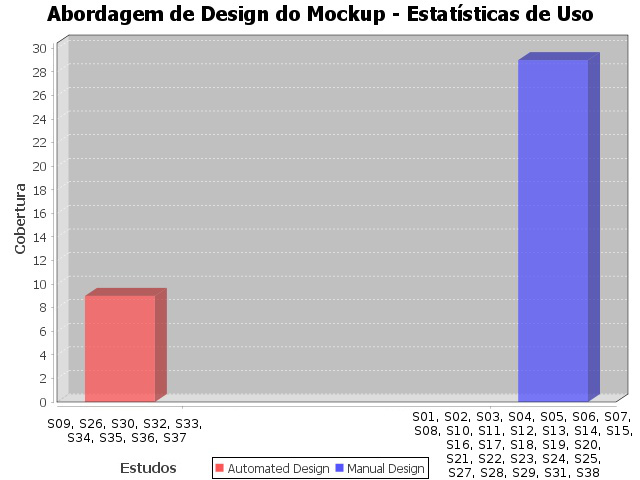
\includegraphics[width=240pt]{./imgs/DesignApproach.jpeg}
    \caption{Distribuição dos Estudos por Abordagem de Design.}
    \label{fig:DesignApproach}
\end{figure}

Uma vez definido o framework de comparação, agrupou-se os estudos conforme dois atributos de qualidade das 38 abordagens: 1) automação do design do mockup por meio de programas/scripts para refinamentos de modelos de GUI; e 2) o processo de transformação adotado para a geração do código. 

A Figura~~\ref{fig:DesignApproach} apresenta a distribuição dos trabalhos para design de mockups, assim respondendo a questão de pesquisa RQ02. Os 9 estudos que caracterizam abordagens para "Automated Design" oferecem um diferencial em relação às demais: elas permitem gerar automaticamente representações de front-end, como usar tais representações para gerar outras camadas da aplicação derivadas do MVC.

Para responder a questão de pesquisa RQ03, caracterizou-se as propostas conforme o fluxo de transformação de modelos, como mostrado na Figura~\ref{fig:RefinementFlow}. Pouco menos de metade dos trabalhos (15) apresentam um processo simples, que transforma um modelo de Mockup diretamente para código fonte. Já os 23 demais trabalhos introduzem múltiplas visões para refinamento dos modelos em diversas camadas de aplicação, alternando o modelo de entrada. Todas as abordagens geram código.  





\begin{figure}[t!]
    \centering
    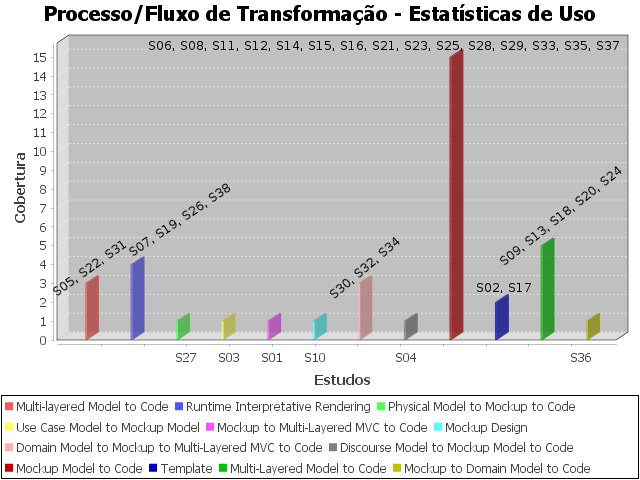
\includegraphics[width=240pt]{./imgs/RefinementFlow.jpeg}
    \caption{Distribuição dos Estudos por Processo de Transformação de Modelos.}
    \label{fig:RefinementFlow}
\end{figure}
 
\subsection{Aplicação em Contextos da Indústria}

Outro ponto que investigamos foi como estas tecnologias vem sendo utilizadas na indústria, respondendo assim a questão de pesquisa RQ04. Encontramos que, dentre 38 artigos, apenas sete das pesquisas apresentam estudos de viabilidade das ferramentas em contextos industriais: \{S10, S26, S30-S32, S34 e S38\}. Cabe ressaltar que os estudos \{S30-S32 e S34\} apresentam relatos de aplicação em mais de um contexto industrial. Ou seja, são relatados em projetos de software de vários domínios, cujas tecnologias utilizadas para implementação também variam em termos de APIs, padrões arquiteturais e de codificação. Portanto, são poucos os casos em que o objetivo de se obter independência de plataformas é comprovadamente observado em projetos de software executados por meio de MDWE.

Essa observação é um tanto paradoxal para este tipo de pesquisa. Em geral, as abordagens de MDWE são motivadas sobre o guarda-chuva de desenvolvimento multi-plataforma (independente delas), mas a maioria dos relatos 31 não corroboram com sua comprovada efetividade na prática como uma solução deste problema. Um dos motivos por esta pequena amostra, i.e., de três relatos de contextos envolvendo desenvolvimento multi-plataforma, pode ser o fato de que artigos tratando de DSLs oferecem uma contribuição focada em termos de abstração, e não de prática. 

Para remover esta limitação, que nos impede de realizar uma conclusão definitiva sobre a efetividade das DSLs na prática, é preciso realizar uma segunda revisão do tipo snowballing. Por meio dela, espera-se encontrar os trabalhos dos mesmos autores dos artigos relatados, mas que apresentem estudos observacionais complementares na indústria. %~\cite{Wohlin14}



\section{Ameaças à Validade}
\label{sec:threats}

Este estudo pode sofrer algumas ameaças à validade~\cite{Wohlin12}, que alcançam validades internas, do construtor e da conclusão do estudo como segue:


\textbf{Validade do Construtor:} 
Discute a validade das declarações neste artigo e esgota as propriedades que mostram se ele realmente exerceu o que pretendia declarar. Em primeiro lugar, os Estudos de Mapeamento Sistemático são bem conhecidos por não garantir a inclusão de todos os trabalhos relevantes no campo. Isso pode ser explicado pela limitação dos mecanismos de busca para um conjunto de palavras-chave definidas neste trabalho e pela falta delas nos trabalhos relevantes. A fim de evitar grandes problemas relacionados a essas questões descritas, adotamos cuidadosamente procedimentos rigorosos para recuperar e filtrar os estudos primários. Palavras-chave e seus sinônimos foram definidos de acordo com métodos bem estabelecidos em~\cite{Kitchenham07}. Além disso, incluímos quatro das principais bases de dados científicas e também adicionamos uma etapa chamada "adição por heurística" com o objetivo de contemplar a fase de pesquisa com trabalhos que já sabemos estarem relacionados, mas as etapas iniciais não conseguiram detectar. Em segundo lugar, não podemos assegurar a validade das declarações dos estudos recuperados.% Mesmo que nós decidimos evitar a literatura cinza (nenhum material revisado por pares), alguns trabalhos são originados de workshops e eventos onde o processo de revisão é mais superficial relacionado aos periódicos tradicionais. Por fim, para garantir a remoção apropriada de estudos duplicados, os artigos de todos as bases de busca foram reunidos em um diretório separado antes de filtrarmos os repetidos.

\textbf{Validade Interna:} 
Esse tipo de ameaça se refere à validade da análise realizada. Isto é, se as conclusões derivadas dos dados são internamente válidas. Cada estudo primário identificado implementa sua própria abordagem para design. Para categorizá-los, consideramos a estrutura do fluxo de transformações de modelo para modelo e modelo para código. Com base nessas categorias, procuramos entender cada abordagem e, em seguida, classificá-las, ou seja, mapear cada tipo de transformação com base em categorias de correspondência e de similaridade. Entender e mapear cada técnica pode ser visto por si só como uma ameaça à validade. Com isso em mente, procuramos mitigar esse risco discutindo e analisando de perto todos os autores do artigo. Além disso, uma preocupação sempre presente durante todo o estudo era garantir que os estudos primários selecionados fossem consistentemente identificados e analisados. Para isso, investimos cuidadosamente um enorme esforço para filtrar os estudos primários.

\textbf{Validade da Conclusão:} 
Essas ameaças estão estritamente relacionadas a problemas que podem afetar
confiabilidade de nossas conclusões. Primeiro, seguimos rigorosamente as etapas fornecidas pelo protocolo de estudo de mapeamento sistemático bem difundido~\cite{Kitchenham07}. %Em segundo lugar, descrevemos extensivamente todas as etapas para conduzir o estudo de mapeamento sistemático, também fornecemos o link do repositório para o banco de dados Mendley, onde todos os resultados das etapas de estudos de filtragem são fornecidos [Mendley 2016].
Finalmente, todas as conclusões deste artigo foram feitas após a coleta dos resultados, evitando a taxa de erro e de "fishing~\cite{Kitchenham07}.




\section{Conclusões e Trabalho Futuros}
\label{sec:conclusions}

Este artigo apresentou um mapeamento de literatura em MDWE front-ends, caracterizando de forma resumida o total de 38 propostas. Por meio deste mapeamento, encontramos que a pesquisa dirigida para características estruturais de DSLs, como design de componentes que embutem semântica de ações neste contexto, é madura. Ou seja, em termos de representatividade, as DSLs existentes cobrem, se não todas, grande parte das necessidades para design de componentes de web front-ends das plataformas de desenvolvimento atuais. No entanto, as abordagens para design automatizado ainda estão no seu início. Portanto, pretende-se ampliar este estudo para os seguintes complementos:


%1) Um consenso observado nos estudos é que DSLs para representação de front-ends web são essenciais para desenvolvimento rápido de aplicações em multi-plataformas. Além disso, DSLs construídas com base em design automático permitem capturar as necessidades do cliente nas fases preliminares de desenvolvimento de software, o que é importante para a execução da disciplina da Engenharia de Software denominada Verificação e Validação (V\&V). Assim, em trabalhos futuros pretende-se explorar técnicas de V\&V alinhadas com design automático, avaliando também se ferramentas de nosso grupo de pesquisa como a MockupToME~\cite{Basso16JSS}, contribuem para a execução de atividades nessa disciplina;

1) A literatura carece de estudos de viabilidade do MDWE conduzidos em contextos de Fábricas de Software. Ao longo de nossa investigação, percebeu-se que poucos trabalhos discutiram como a indústria recebeu estas tecnologias. Isso é um tanto decepcionante, já que tais pesquisas são motivadas em problemas da indústria de software. Assim, %como seguimento dos estudos empíricos discutidos em~\cite{Basso15IJWET}, 
pretende-se estudar como diferentes atributos de qualidade, na transferência de tecnologia de MDWE, afetam a aceitação destes produtos no mercado por determinados perfis de times de desenvolvimento, e; %. Por exemplo, times ágeis podem ter preferências por determinados atributos de qualidade de ferramentas de MDWE em relação a outras, e;

2) Por fim, deve-se ampliar o relato deste mapeamento. Por motivos de formato do relato, e como forma de caracterização da área de pesquisa, pôde-se apenas conceituar as propostas existentes. Assim, ficou faltando elementos importantes de um mapeamento sistemático como uma análise comparativa das características estruturais das DSLs encontradas. Também pretendemos aplicar os critérios de representação de artefatos de MDE, que são recursos intensivos em conhecimento que influenciam na tomada de decisão para transferência de tecnologia da área. Portanto, como próximo trabalho, pretende-se apresentar esta parte complementar de nosso estudo.



%\bibliographystyle{ACM-Reference-Format}
\bibliographystyle{abbrv}
\bibliography{sbc-template}
\end{document}





